%; whizzy chapter -dvi
% -initex iniptex -latex platex -format platex -bibtex jbibtex -fmt fmt
% 以上 whizzytex を使用する場合の設定。

%     Tokyo Debian Meeting resources
%     Copyright (C) 2012 Junichi Uekawa
%     Copyright (C) 2012 Nobuhiro Iwamatsu

%     This program is free software; you can redistribute it and/or modify
%     it under the terms of the GNU General Public License as published by
%     the Free Software Foundation; either version 2 of the License, or
%     (at your option) any later version.

%     This program is distributed in the hope that it will be useful,
%     but WITHOUT ANY WARRANTY; without even the implied warranty of
%     MERCHANTABILITY or FITNESS FOR A PARTICULAR PURPOSE.  See the
%     GNU General Public License for more details.

%     You should have received a copy of the GNU General Public License
%     along with this program; if not, write to the Free Software
%     Foundation, Inc., 51 Franklin St, Fifth Floor, Boston, MA  02110-1301 USA

%  preview (shell-command (concat "evince " (replace-regexp-in-string "tex$" "pdf"(buffer-file-name)) "&"))
% 画像ファイルを処理するためにはebbを利用してboundingboxを作成。
%(shell-command "cd image201211; ebb *.png")

%%ここからヘッダ開始。

\documentclass[mingoth,a4paper]{jsarticle}
\usepackage{monthlyreport}

% 日付を定義する、毎月変わります。
\newcommand{\debmtgyear}{2012}
\newcommand{\debmtgmonth}{11}
\newcommand{\debmtgdate}{17}
% (+ (* (- 2012 2005) 12) 10 -1) started from zero
\newcommand{\debmtgnumber}{94}

\begin{document}

\begin{titlepage}
\thispagestyle{empty}
% タイトルページ:編集必要な部分は最初のマクロに飛ばすこと

\vspace*{-2cm}
第\debmtgnumber{}回 東京エリア Debian 勉強会資料\\
\hspace*{-2cm}

\includegraphics{image2012-natsu/dotdeb.pdf}\\
\hfill{}\debmtgyear{}年\debmtgmonth{}月\debmtgdate{}日

% ここはアップデートすること
% 全角文字にしないとフォントのサイズが合わないので注意
% TODO(uekawa): なんでそうなるのか確認
\rotatebox{10}{\fontsize{32}{32} {\gt 特集: Linux perf}}\\
\rotatebox{10}{\fontsize{32}{32} {\gt 特集: Bluetooth Tether}}\\

\vspace*{-2cm}
\hfill{}
\includegraphics[height=6cm]{image200502/openlogo-nd.eps}
\end{titlepage}

% Title should be in Japanese text so that we can use it as lint for PDF shiori.
\dancersection{はじめに}{上川 純一}

\begin{multicols}{2}
 

 今月のDebian勉強会へようこそ。これからDebianの世界にあしを踏み入れると
 いう方も、すでにどっぷりとつかっているという方も、月に一回Debianについ
 て語りませんか?

 Debian勉強会の目的は下記です。

 \begin{itemize}
 \item \underline{Debian Developer} (開発者)の育成。
 \item 日本語での「\underline{開発に関する情報}」を整理してまとめ、アップデートする。
 \item \underline{場}の提供。
 \begin{itemize}
  \item 普段ばらばらな場所にいる人々が face-to-face で出会える場を提供
	する。
  \item Debian のためになることを語る場を提供する。
  \item Debianについて語る場を提供する。
 \end{itemize}
 \end{itemize}		

 Debianの勉強会ということで究極的には参加者全員がDebian Packageをがりがり
 と作るスーパーハッカーになった姿を妄想しています。情報の共有・活用を通し
 て Debianの今後の能動的な展開への土台として、「場」としての空間を提供す
 るのが目的です。

\end{multicols}

\newpage

\begin{minipage}[b]{0.2\hsize}
 \definecolor{titleback}{gray}{0.9}
 \colorbox{titleback}{\rotatebox{90}{\fontsize{80}{80} {\gt デビアン勉強会} }}
\end{minipage}
\begin{minipage}[b]{0.8\hsize}
\hrule
\vspace{2mm}
\hrule
\begin{multicols}{2}
\tableofcontents
\end{multicols}
\vspace{2mm}
\hrule
\end{minipage}

\dancersection{事前課題}{上川 純一}

今回の事前課題は以下です:
\begin{enumerate}
 \item Debian で今いまいちサポートされていない機能、いけてない実装について語ってください。
\end{enumerate}
この課題に対して提出いただいた内容は以下です。
\begin{multicols}{2}
{\small
%; whizzy-master ../debianmeetingresume201211.tex
% $B0J>e$N@_Dj$r$7$F$$$k$?$a!"$3$N%U%!%$%k$G(B M-x whizzytex $B$9$k$H!"(Bwhizzytex$B$,MxMQ$G$-$^$9!#(B
%

\begin{prework}{ koedoyoshida }

\begin{itemize}
 \item Wheezy$B%$%s%9%H!<%i$N%Q!<%F%#%7%g%s9=@.;~$N%G!<%?>C5nBT$A;~4V!#(B
 $B0E9f2=%Q!<%F%#%7%g%s$r:n$m$&$H$9$k$H2L$F$7$J$/BT$?$5$l$k!#(B
 \item 
 Wheezy$B$NJI;f!#$$$1$F$J$$46$8$G(BOSC$B$H$+$NE8<($GE,Ev$J$b$N$rA*$V$N$,LLE]$G7k6I(Bsqueeze$B$d(BDebian$B$N(B($B2a5n$N(B)$B%8%'%M%j%C%/$J$b$N$rA*$V$3$H$K(B...
 \item 
 $B%G%P%C%0%7%s%\%k$r4^$s$@%P%$%J%j$,$J$$!#(B
 $B0JA0BgE}0l$G4d>>$5$s$,H/I=$7$F$$$?OC$,?J$s$G$$$k$H$&$l$7$$!#(B
\end{itemize}

\end{prework}

\begin{prework}{ $B%-%?%O%i(B }

$B;d$,;HMQ$9$kHO0O$G$O$"$j$^$;$s!#(B

\end{prework}

\begin{prework}{ MATOHARA }

$B$"$^$j;W$$$D$+$J$$$G$9$,!"?M$HOC$r$7$F$$$k$H$-0J2<$N$h$&$J$3$H$r8@$o$l$?$3$H$,$"$j$^$9!#(B
\begin{itemize}
 \item 
 Debian$B$O5,DjCM$N@_Dj$,$$$1$F$J$$$N$G@_Dj$rBt;3$$$8$i$J$$$H1?MQ=PMh$J$/$F9)?t$,L5BL$K3]$+$k(B
 \item 
 Debian$B$O%$%s%9%H!<%k$,Fq$7$$(B
\end{itemize}
$B6qBNNc$rJ9$1$J$+$C$?$N$G$9$,!"@_Dj$K$D$$$F$O@i:9K|JL$J$N$G$=$N?M$K$H$C$F(B
 $B8~$$$F$$$J$+$C$?$+$i$H8@$C$F%@%a$+$H$$$&$H$=$&$G$O$J$$$H;W$$$^$9!#(B
$B$7$+$7!"(BopenSUSE $B$N(BYaST $B$O0l85E*$K4IM}$G$-$FJXMx$=$&$@$J$H$O;W$$$^$9!#(B
$B%$%s%9%H!<%k$,Fq$7$$$H$$$&$N$b@N$N%$%a!<%8$J$N$+8=:_$N$3$H$r8@$C$F$$$k$NITL@$J$N$G$9$,!"%G%9%/%H%C%W8~$1$N%G%#%9%H%j%S%e!<%7%g%s$KHf$Y$k$HA*Br;h$,B?$$$N$GFq$7$/46$8$i$l$k$N$+$b$7$l$^$;$s!#(B

\end{prework}

\begin{prework}{ $BNkLZ?rJ8(B }

$B8=:_$O2~A1$7$F$$$k$+$b$7$l$^$;$s$,!"0lIt(Bkernel$B$N%Q%C%1!<%8$K$h$C$F$O(Bdbg$B%Q%C%1!<%8$,L5$$$b$N$,$"$C$?$j$7$F!":$$C$?7P83$,$"$j$^$7$?!#(B
\end{prework}

\begin{prework}{ $BLnEg!!5.1Q(B }

Debian$B$G$$$1$F$$$J$$5!G=!?<BAu$H$$$o$l$k$H!"(B

\begin{itemize}
 \item  ifupdown$B%Q%C%1!<%8(B
 \item  Solaris10$B0J>e$G$$$&$H$3$m$N(BFMD$B$H$+!"(BSVC$BM_$7$$!#(B
 \item  $B%$%s%9%H!<%i$G(B'/'$BA4It(BBTFS$B$H$$$&$NA*Br2DG=$G$7$?$C$1!)(B
 \item  WEB$BMm$_$G!":G?7(BWEB$B3+H/4X780l<0$N%Q%C%1!<%8%j%]%8%H%j$H$$$&$N$,M_$7$$5$$,$9$k!J(BWEB$B%7%9%F%`$GN.9T$j$b$N$d$i!"NI$/;H$o$l$F$$$=$&$J%P!<%8%g%s$N%=%U%H$KFC2=$7$?%j%]%8%H%j!#$=$l$J$i(Bexperimental$B$7$+B8:_$7$J$$$H$+$G$b%$%$!*!K(B
 \item  Debian$B$H$O$A$g$C$H%:%l$F$k$+$b$7$l$^$;$s$,!"(Bsynaptic$B$O(B...iTunes$B$_$?$$$K$J$C$F$[$7!<(B
\end{itemize}

$B$H8@$$$?$$J|Bj8@$C$F$_$?!#(B
\end{prework}

\begin{prework}{ $B>e@n=c0l(B }

Android $BMQ$N(BADB$B%3%^%s%I$H$+$,I8=`$GF~$C$F$$$k$H4r$7$$$J$!!#(B
\end{prework}

\begin{prework}{ yamamoto }

Debian $B$NM}A[$H?.G0$OBg9%$-$J$s$G$9$,!">/$75$$K$J$kE@$b$"$j$^$9!#(B

$BNc$($P(B Debian-Installer $B$K$O(B non-free $B$GHRI[$5$l$F$$$k(B firmware $B%Q%C%1!<%8$,4^$^$l$F$$$J$$E@$J$I$G$9!#(Bnon-free $B$N%Q%C%1!<%8$O!"MM!9$JM}M3$G(B non-free $B$KJ,N`$5$l$F$$$k$o$1$G$9$,!"$=$N0l$D$K%F%-%9%H$N%=!<%9$,B8:_$7$J$$$?$a!"$H$+$$$&M}M3$b$"$j$^$9!#(B

$BJL$K!V(Bnon-free $B$K$9$k$J!W$H$+<gD%$7$?$$$o$1$G$O$J$$$N$G$9$,!"HRI[$N@)8B$NL5$$%Q%C%1!<%8$^$G!V(Bnon-free $B$@$+$i!W$H!"<}O?$r5q@d$9$k$N$O>/!9$d$j$9$.$G$O$J$$$+$H9M$($F$$$^$9!#(B
\end{prework}

\begin{prework}{ $BLn<s(B }

\begin{itemize}
 \item $B%Q%C%1!<%8$N%j%9%H%"$K(Bdpkg --get-selections$B$O$A$g$C$HHyL/(B
 \item aptitude-run-state-bundle$B$O$$$^$$$AMQES$,$o$+$i$J$$(B
 \item stable$B$K$?$^$K;H$$J*$K$J$i$J$$%Q%C%1!<%8$,$"$k(B
       \begin{itemize}
	\item $B8E$9$.$k$+$i$H$+(B($BNc(B: lxc)
       \end{itemize}

 \item $B%Q%C%1!<%8$N%H%i%s%6%/%7%g%s$,M_$7$$(B
       \begin{itemize}
	\item $B0lEY%$%s%9%H!<%k$7$F$_$F$*$+$7$+$C$?$i(Brevert
	\item $BLdBj$J$1$l$P(Bcommit$B$_$?$$$J(B
       \end{itemize} 
\item multiarch$B$OF3F~$7$FK\Ev$KNI$+$C$?$N$+(B?
\end{itemize}

\end{prework}

\begin{prework}{ $BF|HfLn(B $B7<(B }

$B;H$$$3$_$,B-$j$F$J$$$N$+$b$7$l$^$;$s$,!"(B
$BMzNr4IM}%7%9%F%`$KJ]B8$5$l$F$$$k(Btree$B$r(B
debian$B%Q%C%1!<%8$H$7$F(B build $B$7$?$j(B
install $B$7$?$j$9$k$H$-$KJXMx$J%D!<%k$,(B
$B$"$^$jL5$$$N$+$b$H;W$$$^$7$?!#(B

\end{prework}

\begin{prework}{ dictoss($B?yK\!!E5=<(B) }

iptables$B$N%3%^%s%I0z?t$,B>$N(BOS$B$H0c$&$h$&$J46$8$,$9$k!#$=$N$?$a(Biptables$B$N=i?4<T$,(Bweb$B$GD4$Y$?%3%^%s%I$r<B9T$7$F$b9=J8%(%i!<$G$O$8$+$l$F?I$$!#(B
\end{prework}

}
\end{multicols}

\dancersection{Debian Trivia Quiz}{上川純一}

ところで、みなさん Debian 関連の話題においついていますか?Debian関連の話
題はメーリングリストをよんでいると追跡できます。ただよんでいるだけではは
りあいがないので、理解度のテストをします。特に一人だけでは意味がわからな
いところもあるかも知れません。みんなで一緒に読んでみましょう。

今回の出題範囲は\url{debian-devel-announce@lists.debian.org} や \url{debian-devel@lists.debian.org}に投稿された
内容とDebian Project Newsからです。

\begin{multicols}{2}
%; whizzy-master ../debianmeetingresume201211.tex
% $B0J>e$N@_Dj$r$7$F$$$k$?$a!"$3$N%U%!%$%k$G(B M-x whizzytex $B$9$k$H!"(Bwhizzytex$B$,MxMQ$G$-$^$9!#(B
%

\santaku
{FTP master $B$K$"$?$i$7$/;22C$7$?$N$O(B}
{iwamatsu}
{ansgar}
{bdale}
{B}
{Ansgar $B$,?7$7$/;22C$7$^$7$?!#(Bmhy, joerg, ansgar $B$N;0?MBN@)$K(B}

\santaku
{pdiff$B$G2?$,2~A1$5$l$?$+(B}
{$B:GBg(B2$B$D$N(BDiff$B$r%@%&%s%m!<%I$9$l$PNI$$$h$&$KJQ99$K$J$C$?(B}
{$B0lF|(B10$B8D$E$D(BDiff$B$r@8@.$9$k$h$&$K$J$C$?(B}
{Diff$B$C$F$J$K$=$l$*$$$7$$$N!)(B}
{A}
{apt-get update $B$NCY$5$,%^%7$K$J$j$^$9$M!#(B}

\santaku
{CTTE 573745 $B$G2?$,7hDj$5$l$?$+(B}
{Mattias Klose $B%/%S(B}
{python $B=*N;$N$*CN$i$;(B}
{$B$_$s$JCgNI$/$7$h$&$M(B}
{C}
{python $B$N%a%s%F%J$N%3%_%e%K%1!<%7%g%sITB-$K$D$$$F$N5DO@$O7k6I$_$s$JCgNI(B
$B$/$7$^$7$g$&$H$$$&7kO@$K$J$j$^$7$?$M!#(B}

\santaku
{$B?7$7$/(BFront Desk$B$N%a%s%P!<$K$J$C$?$N$O(B}
{Kouhei Maeda}
{Iwamatsu}
{Jonathan Wiltshire}
{C}
{4$B?M$K$J$j$^$7$?!'(B
 Bernd Zeimetz      (bzed)
 Enrico Zini        (enrico)
 Jan Hauke Rahm     (jhr)
 Jonathan Wiltshire (jmw)
}

\santaku
{debian installer 7.0 beta3 $B$N?75!G=$G$O$J$$$N$O$I$l$+(B}
{ipv6}
{UEFI}
{grub2}
{C}
{}

\santaku
{}
{}
{}
{}
{}
{}
\santaku
{}
{}
{}
{}
{}
{}
\santaku
{}
{}
{}
{}
{}
{}
\santaku
{}
{}
{}
{}
{}
{}

\end{multicols}

%-------------------------------------------------------------------------------
\dancersection{Android 携帯でBluetooth Tethering}{上川純一}
%-------------------------------------------------------------------------------
\index{bluetooth}
\index{bluetooth tethering}
\index{tethering}

\subsection{はじめに}

最近のAndroid携帯もパソコンもBluetoothに対応しています。そしてBluetooth
profileであるPANやDUNに対応しているものも多いようです。
Android 4.0あたりで対応するようになったと思われるBluetooth Tetheringを利
用することでAndroid携帯にBluetooth PAN 経由で接続し、Android携帯の回線を
利用して外部のネットワークに接続できるようになります。

WiFi Tetheringのように電力消費が高すぎるので毎回設定でオフにする必要があ
るるということもなく、やUSB Tetheringのように毎回物理的に接続する必要もな
いので便利です。
カバンの中に携帯をいれたまま接続できるので気楽ですよ。

\subsection{設定方法}

Android携帯側ではBluetooth Tetheringをオンにします。
\fgref{fig:android-bt})

\begin{figure}[H]
 \begin{center}
  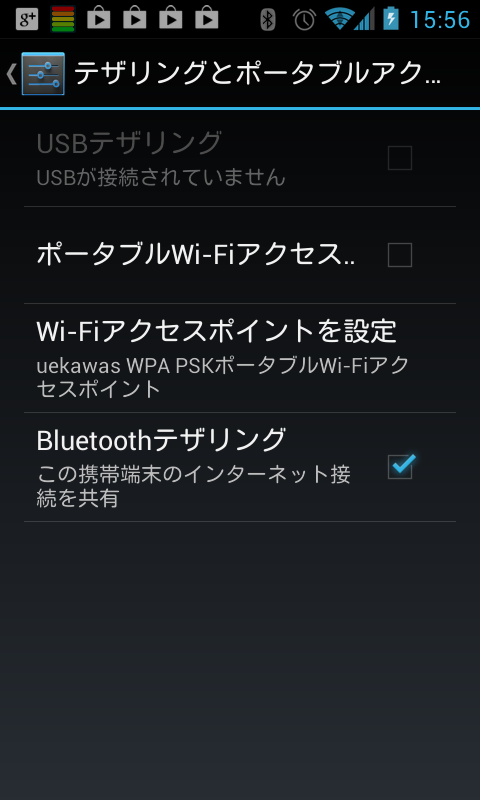
\includegraphics[width=0.3\hsize]{image201211/bt-android.png}
  \label{fig:android-bt}
 \end{center}
\end{figure}

あと、Bluetoothのペアリングを行います。携帯電話側の設定で可視状態にして
おいてGNOMEの設定で追加すればよいでしょう。(\fgref{fig:gnome-bt2})

\begin{figure}[H]
 \begin{center}
  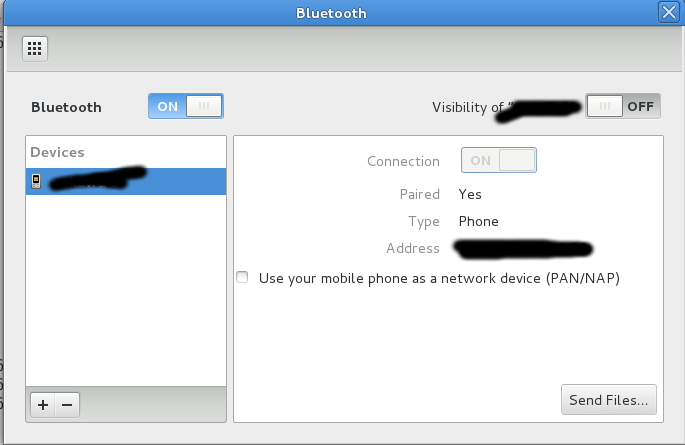
\includegraphics[width=0.5\hsize]{image201211/bt2.png}
  \label{fig:gnome-bt2}
 \end{center}
\end{figure}

一旦設定しておくとネットワークの選択候補にMobile Broadbandというのが現れ
てそこで携帯電話のBluetooth PAN接続が選択できるようになります。

\begin{figure}[H]
 \begin{center}
  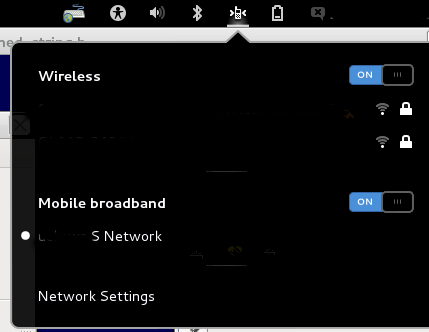
\includegraphics[width=0.5\hsize]{image201211/bt1.png}
  \label{fig:gnome-bt1}
 \end{center}
\end{figure}

\subsection{ネットワーク構成}

Linux 側からはbnep0 デバイスとして見えます。複数マシンから接続するとそれ
ぞれが別のサブネットに接続されるっぽいのでお互いに通信はできないようです。
WiFi Tetheringだと同じサブネットにつながるので個人的にはウェブサーバーと
クライアントを接続するためのハブとして便利に利用していたのですが、そうい
う使い方はできないようです。

\begin{commandline}
bnep0     Link encap:Ethernet  HWaddr 
          inet addr:192.168.46.43  Bcast:192.168.46.255  Mask:255.255.255.0
\end{commandline}

\subsection{まとめ}

Bluetooth PANは便利、ということでした。ただ、なぜだか日本の携帯電話は
Bluetooth PANに対応してないものが多く、また海外携帯の日本モデルはその機能
を削ってたりするものがあります\footnote{例:筆者の所有するGalaxy Nexus
DoCoMo版}。ここはぜひBluetooth PAN対応じゃない携帯電話は購入しないことで
消費者の意見を表明してください。

%-------------------------------------------------------------------------------
\dancersection{perf でパフォーマンスチューニング}{上川純一}
%-------------------------------------------------------------------------------
\index{perf}
\index{linux perf}
\index{Performance Counters}

\subsection{はじめに}

最近のたいていのCPUにはHardware Performance Counters という仕組みがあり、特定のイ
ベントが一定回数発生したらある処理をするという事ができるようになっていま
す。それを利用してプロファイラーが実装できて、プログラムのパフォーマンス
ボトルネックの発見に役立てることができます。
昔は oprofile を使っていたのですが、最近のLinux カーネルでは perf という
仕組みを使うのが主流のようです。

カーネル側のサポートは標準で入っています。コマンドラインの perf コマンド
は linux-base パッケージにはいっていてたいていの環境では標準でインストー
ルされているようにみえるのですが実体はカーネルにあったバージョンを追加で
インストールする必要があります。例えば、linux 3.2 だと linux-tools-3.2 を
インストールすることになります。

\begin{commandline}
 $ uname -r
3.2.0-3-amd64
 $ sudo apt-get install linux-tools-3.2
\end{commandline}
\index{linux-tools-3.2}

デバッグシンボルがあると関数名とかがきれいに出る気がするので利用している
ライブラリのデバッグシンボルもいれておくとよいでしょう。標準ライブラリは
いれておきましょう。

\begin{commandline}
 $ sudo apt-get install libc6-dbg libstdc++6-4.7-dbg
\end{commandline}
%$

\subsection{perf stat}

プログラム単体の実行時間を計測してレポートしてくれるコマンドとして timeコ
マンドがありますが、その代わりにつかえそうなツールとして、 perf stat があ
ります。最近のCPUは負荷によってCPU周波数が変わり、そういうシステムにおい
てパフォーマンスの測定のために実行時間だけを計測するというのは適切ではな
いのですが、perf statはそれ以外に必要そうな値を計測してくれるので便利です。

\begin{commandline}
$ perf stat ./apt-index-cmd debian_dists_sid_main_binary-amd64_Packages debian > /dev/null
 Performance counter stats for './apt-index-cmd debian_dists_sid_main_binary-amd64_Packages debian':

       1741.828818 task-clock                #    0.997 CPUs utilized          
               165 context-switches          #    0.000 M/sec                  
                 6 CPU-migrations            #    0.000 M/sec                  
            27,392 page-faults               #    0.016 M/sec                  
     4,990,934,326 cycles                    #    2.865 GHz                     [83.29%]
     1,681,297,382 stalled-cycles-frontend   #   33.69% frontend cycles idle    [83.27%]
     1,096,373,883 stalled-cycles-backend    #   21.97% backend  cycles idle    [66.62%]
     7,738,965,303 instructions              #    1.55  insns per cycle        
                                             #    0.22  stalled cycles per insn [83.51%]
     1,784,494,907 branches                  # 1024.495 M/sec                   [83.49%]
        32,701,183 branch-misses             #    1.83% of all branches         [83.32%]

       1.746581711 seconds time elapsed
\end{commandline}
  
\subsection{perf record}

perf record コマンドはプロファイル情報を記録する命令です。パラメータとし
て指定したコマンドをそのまま実行して、カレントディレクトリに perf.dataファ
イルを作成します。後に perf report などでそのプロファイルデータを確認する
ことができます。

\begin{commandline}
$ perf record ./apt-index-cmd debian_dists_sid_main_binary-amd64_Packages  debian > /dev/null
[ perf record: Woken up 1 times to write data ]
[ perf record: Captured and wrote 0.087 MB perf.data (~3800 samples) ]
$ ls -l perf.data
-rw------- 1 dancer dancer 93560 10月 10 07:03 perf.data

\end{commandline}

perf record -g オプションをつけるとコールグラフ情報も記録するようです。

デフォルトは一秒1000サンプルとるようなので、プログラムの実行時間に応じて
サンプル数を適当に調整しましょう。 例えば全体で実行が一秒で終わってしまう
プログラムの場合は-F 10000 をつけてみるとよりサンプル数がとれていいかもし
れません。

\subsubsection{gcc のコンパイルオプションの検討}

gcc でソースコードコンパイルするときに、-g オプションをつけるとデバッグ情
報がつきます。関数シンボルの情報とか行数とかソースコードとかが得られるの
でこれは多分重要。

コールグラフがあまりないなぁと思ったら最適化のしすぎとスタックトレースの
とりにくさを疑ってみましょう。

通常最適化オプション -O2 をつけてコンパイルしますが、amd64 の場合、gcc で
-O2 をつけてコンパイルするとフレームポインタがなくなってスタックトレース
を取得しにくくなっています。libunwind使えば取得できるはずですが、多分
perfはカーネル空間でスタックトレースをとっているのでそうなってないっぽい
です。対策として若干オーバーヘッドがありますが、-fno-omit-frame-pointer
を指定すると、フレームポインタを操作するコードを生成してくれます

C++でファンクションオブジェクトとかテンプレートプログラミングしまくってい
ると、関数がほとんどインライン展開されてしまい、コールグラフに現れる部分
が少なくなります。理解不能になってきたらたまに -O あたりでコンパイルして
スタックトレースを見てみましょう。

\subsection{perf report}

perf report コマンドは取得したプロファイルデータを可視化するコマンドです。
テキストコンソールメニュー形式になっていて、気になるシンボルを選択してソー
スコードのアノテーションを見ることができます。どのソースコードの行に対応
するアセンブラのどの命令でCPU処理時間を費やしたのかを表示してくれます。

\begin{commandline}
$ perf report
Events: 1K cycles                                                              
 18.65%  apt-index-cmd  apt-index-cmd        [.] available_parser::AptIndexSpiri
  7.38%  apt-index-cmd  libc-2.13.so         [.] _int_malloc
  6.64%  apt-index-cmd  libc-2.13.so         [.] malloc
  5.17%  apt-index-cmd  libstdc++.so.6.0.17  [.] std::string::_M_replace_aux(uns
  4.03%  apt-index-cmd  libc-2.13.so         [.] _int_free
  4.02%  apt-index-cmd  libstdc++.so.6.0.17  [.] __cxxabiv1::__vmi_class_type_in
  3.81%  apt-index-cmd  libstdc++.so.6.0.17  [.] std::string::_M_mutate(unsigned
  3.59%  apt-index-cmd  libstdc++.so.6.0.17  [.] std::ctype<char> const& std::us
  3.00%  apt-index-cmd  libc-2.13.so         [.] __strcmp_sse42
  2.74%  apt-index-cmd  apt-index-cmd        [.] boost::detail::function::functi
  2.72%  apt-index-cmd  libstdc++.so.6.0.17  [.] __dynamic_cast
  2.67%  apt-index-cmd  libc-2.13.so         [.] free
  2.46%  apt-index-cmd  libc-2.13.so         [.] __memcmp_sse4_1
\end{commandline}

ここでエンターをおすと次が表示され

\begin{commandline}

available_parser::AptIndexSpirited::MakeIndex()::{lambda(std::vector<char, std::
    0.00 :          40368a:       je     4036ac <available_parser::AptIndexSpir
         :                                                                     
         :          const std::string& get() const { return my_string_; }      
         :                                                                     
         :          // for 'map' comparison.                                   
         :          bool operator<(const OrderedHashedString& b) const {       
         :            if (ordered_hash_ == b.ordered_hash_) {                  
    2.87 :          40368c:       mov    0x28(%rbx),%rdx                       
         :              return my_string_ < b.my_string_;                      
         :            } else {                                                 
         :              return ordered_hash_ < b.ordered_hash_;                
   34.96 :          403690:       cmp    %rbp,%rdx                             
    1.43 :          403693:       setb   %cl                                   
         :                                                                     
         :          const std::string& get() const { return my_string_; }      
         :                                                                     
         :          // for 'map' comparison.                                   
         :          bool operator<(const OrderedHashedString& b) const {       
         :            if (ordered_hash_ == b.ordered_hash_) {                  
  
 \end{commandline}

\subsubsection{C++ のコードの場合}

C++でテンプレートを活用しているコードを眺める場合、perf report のTUIイン
タフェースだと関数名が十分表示されないなと悩むことになります。とりあえず
TUIじゃないインタフェースにするともっと表示されますが、いまいち全体は表示
できません。

たとえば関数名がこのように途中で切れてしまいます。まだ僕は回避方法を発見して
いません。

\begin{commandline}
 void
 MeasureRaw<std::unordered_map<boost::iterator_range<__gnu_cxx::__normal_iterator<char
 const*, std::string> >, int,
 RangeHash<boost::iterator_range<__gnu_cxx::__normal_iterator<char
 const*, std::string> > >,
 RangeEqualTo<boost::iterator_range<__gnu_cxx::__normal_iterator<char
 const*, std::string> > >,
 std::allocator<std::pair<boost::iterator_range<__gnu_cxx::__normal_iterator<char
 const*, std::string> > const, int> > >, __gnu_cxx::__normal_iterator
\end{commandline}

\subsubsection{おわりに}

一番基本的なPerfの使い方を紹介しました。sudo perf listの出力を確認すると
ハードウェアのいろいろなカウンタだけでなくカーネルが提供しているさまざま
なトレースポイントでのカウンタがあるのがわかります。どう使うか、夢は広が
りますね。

\begin{thebibliography}{98}
 \bibitem{perfman} perf(1) ``perf -- perfomance analysis tools for Linux''
	 manual page. perf\_{}3.2-report(1), etc.
\bibitem{perfwikitutorial} ``Tutorial -- Linux kernel profiling with
	perf'', 
	\url{https://perf.wiki.kernel.org/index.php/Tutorial}

\end{thebibliography}

\dancersection{systemd}{岩松 信洋}
\index{systemd}

\subsection{はじめに}
世の中の主要なLinuxディストリビューションは SysVinit の init scripts から
他のinit システムに移行しつつあります。
FedoraやArch Linuxがsystemd に移行を始めたということもあり、一部で盛り上がっている
(阿鼻叫喚ともいう)ようです。
まさか いまだに SysVinit を使っている Debian勉強会参加者がいるとは思えませんが、
盛り上がっているようなのでDebianとSystemdについてまとめてみました。

\subsection{systemdとは?}

RedHat に勤めている Lennart Poettering 氏によって開発されている init の代替プログラムです。
実際には init の代替だけではなく、Linux のサービス(デーモン)管理フレームワークとなっ
ています。
%Linux カーネル用のデバイス管理ツールである udev が systemd のソースにマージ
%されています。ログシステムもある。将来は cron や acpid などの代替え機能を
%提供する予定らしい。
今までのinitシステムの違いはサービスのプロセス管理を pid ではなく、cgroups を使う点と
サービスの起動をソケットとバスを使う点があります。これらは D-Bus を使って行います。これによってシステム立ち上げ処理をより並列的に行えるようになっています。
また、System V スタイルとBSDスタイルの両方をサポートしています。

開発は freedesktop.org
\url{http://cgit.freedesktop.org/systemd/systemd/}
で行われており、開発は活発で週に一度はバージョンアップしています。
最新バージョンは v195となっています。

\subsubsection{systemd の利点}
systemd は SysVinit と比べて次のような利点があります。

\begin{itemize}
\item 設定が容易。\\
SysVinit はシェルスクリプトで記述していたため、開発者によって書き方が異なります。
よって設定や内容の理解が難しいことがあります。systemd は設定方法や項目等が決まっているため、
設定しやすくなっています。

\item 起動が早い。 \\
シェルに依存していないのとデーモンが並列起動するため起動が早いです。

\item カーネルモジュールの操作、セッション管理、ログ管理、ディスクの暗号化などを
統合。

\end{itemize}

その他、作者による説明を\url{http://0pointer.de/blog/projects/why.html}から参照できます。

\subsection{Debianで使う}

systemd はもちろん Debian でも提供されており、testing / unstable で v44 が
利用できます。最新版とバージョンに差がありますが、アップストリームで
頻繁にバージョンアップするのでバージョンはあまり問題ではありません。
v44 でも systemd を十分に使うことができます。

いまのところ Debianに関する情報は \url{http://wiki.debian.org/systemd}
にまとまっていますが情報が少なく、内容も古いです。

\subsubsection{インストール}
先にも書いたように Debianでは v44 が最新版です。
apt-get / aptitude でインストールできます。

また、Linux カーネルは 2.6.39 以上、devtmpfs, fanotify, autofs4, cgroups が有効になっている
必要があります。

%\begin{commandline}
%$ uname -a 
%Linux debian 3.2.0-4-amd64 #1 SMP Debian 3.2.32-1 x86_64 GNU/Linux
%\end{commandline}
%$

インストールは以下のように実行します。

\begin{commandline}
$ sudo apt-get install systemd
\end{commandline}
%$

以下のパッケージが依存関係でインストールされます。
\begin{commandline}
libsystemd-daemon0
libsystemd-id128-0
libsystemd-journal0
libpam-systemd
\end{commandline}
%$

次に ブートローダにinit指定を追加します。grub を使っている場合、\texttt{/etc/default/grub} の
\texttt{GRUB\_CMDLINE\_LINUX\_DEFAULT} に {\bf init=/lib/systemd/systemd} を追記します。 

\begin{commandline}
変更前:
GRUB_CMDLINE_LINUX_DEFAULT="quiet"
変更後:
GRUB_CMDLINE_LINUX_DEFAULT="quiet init=/lib/systemd/systemd"
\end{commandline} 
%$

変更後、{\bf update-grub}を実行し、grub に設定を反映します。
そしてリブートします。
設定が間違っていないければ systemd で立ち上がるはずです。

\begin{commandline}
$ sudo update-grub
.....
$ sudo reboot 
\end{commandline}
%$

\subsubsection{起動速度}

systemd はアナライザをデフォルトでサポートしています。
起動にかかった時間を確認するには \texttt{systemd-analyze} を実行します。
また、画像で確認したい場合には \texttt{prop} オプションを指定して実行します。
SVG フォーマットで出力されるので、リダイレクトしてファイルに保存します。

\begin{commandline}
$ systemd-analyze 
Startup finished in 1831ms (kernel) + 5669ms (userspace) = 7500ms
$ systemd-analyze plot > systemd-boot.svg
\end{commandline}
%$

試しに自分が常用している環境で起動時間を測定したところ、
SysVinit は約15秒、systemd は約10秒でした。 

\subsection{用語}

systemd を扱っていると専門用語が出てきますので、説明します。

\begin{itemize}
\item ユニット\\
systemd ではデーモンなどの制御対象のことをユニットと呼びます。
ユニットにはサービス、デバイス、マウントポイントなど、いくつかの種類があります。
このユニットはテキストファイルで記述され、\texttt{/lib/systemd/system/} 以下に格納されています。
各ユニットは拡張子を持ち、サービスの場合は\texttt{.service}
となっています。


\begin{table}[htb]
\begin{center}
  \begin{tabular}{ll}
    ユニットの種類 & 説明 \\
    service & デーモン \\
    socket & ソケットによるデーモン \\
    target & multi-user.target \\
    device & udev で管理するデバイス \\
    snapshot & ある時点のinit の状態 \\
    timer & イベントから時間経過 \\
    path & 監視するパス \\
    mount & マウントポイント \\
    swap & スワップ \\
    automaount & 自動マウントポイント \\
  \end{tabular}
\caption{systemd で提供するユニット}
\label{tbl:unit}
\end{center}
\end{table}

mount, swap, automout は起動時に \texttt{/etc/fstab} から自動的に
ユニットを生成してくれます。

\item ターゲット\\
ターゲットとはSysVinit の runlevel 相当のものです。
これはディストリビューションによって異なります。
Debianの場合は以下のようになっています。

\begin{table}[htb]
\begin{center}
  \begin{tabular}{ll}
    run level & systemd のターゲット \\
    0 & poweroff.target \\
    1 & rescue.target \\
    2 - 5 & multi-user.target \\
    6 & reboot.target \\
  \end{tabular}
\caption{run levelとターゲットの対応}
\label{tbl:target}
\end{center}
\end{table}

この他にgraphical.target と emergency.target があります。
前者は X による起動を行うときに呼ばれるターゲット、後者は障害が起こった時に
起動できるようにするためのターゲットです。
ターゲットはカーネルのブートオプションに \texttt{systemd.unit=}で指定でき
ます。何も指定しない場合はdefault.target が呼ばれるようになっています。

\end{itemize}

\subsection{ユニットの操作方法}
systemd に移行した後、デーモン等の制御は /etc/init.d/ 以下を実行するのではなく、{\bf systemctl}
コマンドを使って操作します。以下にユニットの操作方法について説明します。
\index{systemctl}

\subsubsection{起動しているユニットを表示する}

起動しているユニットを表示するには sytemctl を実行します。

\begin{commandline}
$ systemct
...
console-setup.service     loaded active exited        LSB: Set console font and 
cron.service              loaded active running       LSB: Regular background pr
dbus.service              loaded active running       D-Bus System Message Bus
debian-fixup.service      loaded active exited        Various fixups to make sys
exim4.service             loaded active running       LSB: exim Mail Transport A
getty@tty1.service        loaded active running       Getty on tty1
ifup@eth0.service         loaded active exited        ifup for eth0
...
\end{commandline}
%$

\subsubsection{全てのユニットを表示する}

操作できるユニットを表示するには \texttt{--all} を指定します。
 
\begin{commandline}
$ systemctl --all
UNIT                      LOAD   ACTIVE   SUB       JOB DESCRIPTION
proc-sys...misc.automount loaded active   waiting       Arbitrary Executable Fil
dev-cdrom.device          loaded active   plugged       QEMU_DVD-ROM
dev-disk...QM00003.device loaded active   plugged       QEMU_DVD-ROM
dev-disk...QM00001.device loaded active   plugged       QEMU_HARDDISK
dev-disk...2dpart1.device loaded active   plugged       QEMU_HARDDISK
dev-disk...2dpart2.device loaded active   plugged       QEMU_HARDDISK
...
\end{commandline}
%$

\subsubsection{ユニットの状態を確認する}

ユニットの状態を確認するには、\texttt{status} オプションに確認したいユニット名を
指定して実行します。

以下に rsyslog.service ユニットの状態を確認する例を示します。
\begin{commandline}
$ systemctl status rsyslog.service
    Loaded: loaded (/lib/systemd/system/rsyslog.service; enabled)
    Active: active (running) since Wed, 14 Nov 2012 00:37:18 -0800; 22h ago
   Process: 474 ExecStartPre=/bin/systemctl stop systemd-kmsg-syslogd.service (code=exited, status=0/SUCCESS)
  Main PID: 483 (rsyslogd)
    CGroup: name=systemd:/system/rsyslog.service
           └ 483 /usr/sbin/rsyslogd -n -c5
\end{commandline}
%$

これにより、このユニットは \texttt{/lib/systemd/system/rsyslog.service}によって
\texttt{Wed, 14 Nov 2012 00:37:18 -0800}に起動していることが分かります。

\subsubsection{ユニットを起動する}

起動していないユニットを起動するには、 \texttt{start}オプションにユニット名を指定して実行します。
これは \texttt{/etc/init.d/サービス start}と同様の動きとなります。
\begin{commandline}
$ sudo systemctl start ユニット名
\end{commandline}
%$

\subsubsection{ユニットを停止する}

起動しているユニットを停止するには、\texttt{stop}オプションにユニット名を指定して実行します。
これは \texttt{/etc/init.d/サービス stop}と同様の動きとなります。
\begin{commandline}
$ sudo systemctl stop ユニット名
\end{commandline}
%$

\subsubsection{ユニットの設定を再読み込みする}

ユニットの設定を再読み込みするには、\texttt{daemon-reload}オプションにユニット名を指定して実行します。
\begin{commandline}
$ sudo systemctl daemon-reload ユニット名
\end{commandline}
%$

実際に動いているデーモンの設定、例えばhttpdの設定を再読み込みし、再起動するには \texttt{reload}オプションを使います。

\subsubsection{ユニットの自動起動を有効にする}

ユニットの自動起動を有効にするには \texttt{enable} オプションにユニット名を指定して実行します。

有効にすると \texttt{/etc/systemd/system/ターゲット.wants/}に\texttt{/lib/systemd/system/}にあるユニット
へのシンボリックリンクが作成されます。
どのターゲットで自動起動が有効になるかは、ユニットファイルの \texttt{Install}セクションで指定します。

\begin{commandline}
$ sudo systemctl enable ユニット名
\end{commandline}
%$

\subsubsection{ユニットの自動起動を無効にする}

ユニットの自動起動を無効にするには \texttt{disable} オプションにユニット名を指定して実行します。
無効にすると、/etc/systemd/system/ターゲット.wants/にあるシンボリックリンクが削除されます。

\begin{commandline}
$ sudo systemctl disabe ユニット名
\end{commandline}
%$

\subsubsection{ユニットの詳細を確認する}

ユニットの詳細を確認するには \texttt{show} オプションにユニット名を指定して実行します。
これにより指定したユニットと他のユニット、ターゲットの関係などが分かります。

\begin{commandline}
$ sudo systemctl show rsyslog.service
Id=rsyslog.service
Names=syslog.service rsyslog.service
Requires=basic.target
Wants=syslog.socket
WantedBy=multi-user.target
Conflicts=shutdown.target
...                                                           
\end{commandline}                                                                                    
%$

\subsection{ユニットについて}
ユニットには各ユニット間の依存関係を記述することができます。
依存関係の指定として以下があります。

\begin{table}[htb]
\begin{center}
  \begin{tabular}{ll}
    定義 & 説明 \\
    Before & そのユニットの後に起動されるべきユニット。 \\
    After & そのユニットの前に起動されるべきユニット。 \\
    Conflicts & 同時に起動できないユニット。 \\
    Service & ソケットによる起動を行うユニット。 \\
    Sockets & ソケットによるユニットの起動を行う場合のソケット情報 \\
    Wants  & 同時に起動してほしいユニット。成功、失敗は関係ない。\\
    Requires & 同時に起動されなければならないユニット。ユニットの起動が失敗した場合は要求元も失敗する \\
    BindTo & ユニットをグループとしてまとめる。
%ユニットがなくなった場合、グループで指定されているユニットは停止される。\\
  \end{tabular}
\caption{ユニットの依存定義}
\label{tbl:unit-depends}
\end{center}
\end{table}

例えば、default.target の内容は以下のようになっています。
\begin{commandline}
[Unit]
Description=Graphical Interface
Requires=multi-user.target
After=multi-user.target
Conflicts=rescue.target
AllowIsolate=yes
\end{commandline}


このターゲットは
multi-user.targetと同時に起動され、multi-user.targetの後に起動します。
また、rescue.targetと同時に起動できません。

\subsection{まとめ}

Debian でも問題なくsystemd が利用できる環境が整っています。
レガシーなSysVinitは捨て、新しいinitの世界へ足を踏み入れてみてはいかがでしょうか。

\subsection{参考文献}
\url{http://www.slideshare.net/moriwaka/systemd}

% add extra space just to make things fit in 20 pages
\cleartooddpage

\printindex

\cleartooddpage

\vspace*{15cm}
\hrule
\vspace{2mm}

\includegraphics[width=2cm]{image200502/openlogo-nd.eps}
\noindent \Large \bf Debian 勉強会資料\\
\noindent \normalfont \debmtgyear{}年\debmtgmonth{}月\debmtgdate{}日 \hspace{5mm}  初版第1刷発行\\
\noindent \normalfont 東京エリア Debian 勉強会 (編集・印刷・発行)\\
\hrule

\end{document}
